\section{Discussion}
\label{sec:discussion}
Looking back at the results of the experiments, we can see that all feature sets are able to reduce the overall damage of the infrastructure. Where the local-agent is able to reduce only a small amount of damage, the auctioning and knowledge-sharing agents are able to reduce the damage significantly and in a shorter amount of time. 

% \add{Mention the amount of risks detected}
\subsection{Risks Detected}
\label{ssec:risks-detected}
From the figures detailing the unique number of risks detected (figures \ref{fig:risk-count-no-change}, \ref{fig:risk-count-risk-introduction}, \ref{fig:risk-count-growing}, and \ref{fig:risk-count-unstable}) we can see that the local-agent is only able to detect a fraction of the risks that the auctioning and knowledge-sharing agents are able to detect. This is expected as the local-agent cannot share any information with its neighbors, and therefore cannot detect any risks that have an origin outside of its own infrastructure node and software component.

The auctioning agents are able to detect more risks than the knowledge-sharing agents, up to $200\%$ in figure \ref{fig:risk-count-no-change}. 

When comparing the unique number of risks detected to the number of remaining risks in the infrastructure (figures \ref{fig:risk-remaining-no-change}, \ref{fig:risk-remaining-risk-introduction}, \ref{fig:risk-remaining-growing}, \ref{fig:risk-remaining-unstable}) we can see that for the first scenario the auctioning agent detects $150$ out of $600$ risks, which is $25\%$ of the total amount of risks. The knowledge-sharing agent detects $50$ out of $600$ risks, which is $8.3\%$ of the total amount of risks. 

As mentioned before, in the ADRIAN-concept by Mann and Smolka \cite{mann2023ADRIAN} the distance a message can travel is detailed. We believe that the agents would be able to detect more risks if this distance was increased. However, metrics that are collected are not enough to conclude this fully. In the next section (Section \ref{sec:future-research}) this will be discussed further.

% \add{Explain why knowledge-sharing damage output is sometimes better, but more time adaptating is bad}
\subsection{Damage Reduction \& Adaptation Time}
\label{ssec:damage-reduction}
In the results we see that overall knowledge-sharing and auctioning agents tend to perform similarly when looking at the overall damage of the infrastructure. However, when we look at the time spent adapting, we can see that in all cases the knowledge-sharing agents spend almost twice as much time applying adaptations.
Depending on the adaptation, this could mean that the software components running on the infrastructure node could become unavailable for longer periods of time, and that the infrastructure node is unresponsive while applying the adaptations.  In the last scenario (figure \ref{fig:adapting-time-unstable}) we see that the knowledge-sharing agents spends $30$ seconds of the $180$ seconds it was running, which is $16.7\%$ of the time it was running. 

In a real-world scenario this downtime would likely be unfavorable, but should be weighed against the damage that could be done when not applying any adaptations. Applying many adaptations early on could prevent any damage later on, which could be more important than the downtime.


% \add{Mention that adaptation count is the same, but time spent adapting is different}
\subsection{Efficient Adaptations}
\label{ssec:efficient-adaptations}
When looking at the number of adaptations that are applied (figures \ref{fig:proposals-no-change}, \ref{fig:proposals-risk-introduction}, \ref{fig:proposals-growing}, and \ref{fig:proposals-unstable}) we can see that the auctioning and knowledge-sharing agents perform similarly. However, when looking at the time spent adapting (figures \ref{fig:adapting-time-no-change}, \ref{fig:adapting-time-risk-introduction}, \ref{fig:adapting-time-growing}, and \ref{fig:adapting-time-unstable}) we can see that the knowledge-sharing agents spend almost twice as much time adapting. This is an indicator that the auctioning agents are able to apply more efficient adaptations, as they are able to apply the same amount of adaptations in a shorter amount of time, while also reducing the overall damage roughly the same amount.

% \add{Mention the stability of the system}
\subsection{Stability}
\label{ssec:stability}
As the scenarios run their course, we can see that the knowledge-sharing and auctioning agents are able to keep the damage of the infrastructure at a low level. Especially in the Growing Infrastructure scenario (figure \ref{fig:overall-damage-growing-infrastructure}) we see that the damage is kept at a low level, even though the infrastructure is growing. 

The auctioning-agent is able to keep the damage at $10.78\%$ of the damage compared to the local-agent. While the knowledge-sharing agent is able stay at $21.99\%$ of the damage. This is a good result, as the infrastructure is growing, and the agents are able to keep the damage at a low level.

\paragraph*{Small Infrastructure}
During the implementation of the system we noticed that the performance of the different feature-sets was slightly different when the infrastructure was small. The knowledge-sharing agents tends to reach the lowest points almost $50\%$ faster than the auctioning-agent. We believe this to be because of the overhead that is introduced by auctioning. Figure \ref{fig:small-infra-no-change} shows the performance of the different feature-sets in the no-change scenario with a small infrastructure consisting of four infrastructure nodes and two software components.

\begin{figure}[H]
    \centering
        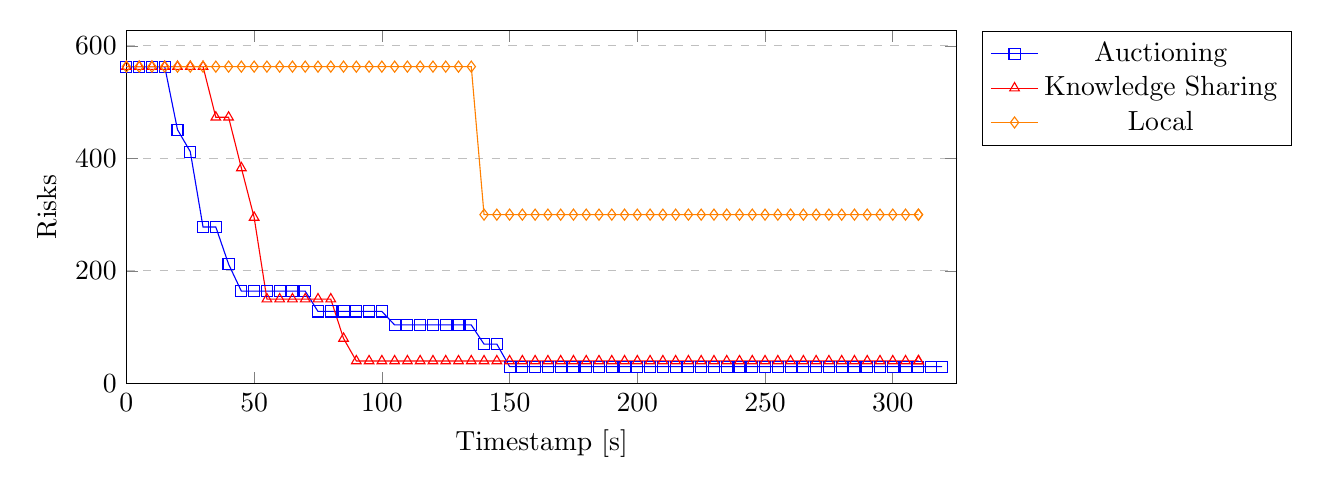
\begin{tikzpicture}
\begin{axis}[
    xlabel={Timestamp [s]},
    ylabel={Risks},
    xmin=0, xmax=325000,
    ymin=0, ymax=627,
    legend pos=outer north east,
    ymajorgrids=true,
    grid style=dashed,
    width=\textwidth,
    height=0.5\textwidth,
    scaled x ticks=base 10:-3,
    xtick scale label code/.code={}
]

	\addplot[color=blue,mark=square] coordinates {
        (0,563)(5000,563)(10000,563)(15000,563)(20000,451)(25000,412)(30000,278)(35000,278)(40000,212)(45000,164)(50000,164)(55000,164)(60000,164)(65000,164)(70000,164)(75000,128)(80000,128)(85000,128)(90000,128)(95000,128)(100000,128)(105000,104)(110000,104)(115000,104)(120000,104)(125000,104)(130000,104)(135000,104)(140000,70)(145000,70)(150000,30)(155000,30)(160000,30)(165000,30)(170000,30)(175000,30)(180000,30)(185000,30)(190000,30)(195000,30)(200000,30)(205000,30)(210000,30)(215000,30)(220000,30)(225000,30)(230000,30)(235000,30)(240000,30)(245000,30)(250000,30)(255000,30)(260000,30)(265000,30)(270000,30)(275000,30)(280000,30)(285000,30)(290000,30)(295000,30)(300000,30)(305000,30)(310000,30)(315000,30)(319272,30)
    };
    \addlegendentry{Auctioning}
	\addplot[color=red,mark=triangle] coordinates {
        (0,563)(5000,563)(10000,563)(15000,563)(20000,563)(25000,563)(30000,563)(35000,473)(40000,473)(45000,383)(50000,295)(55000,150)(60000,150)(65000,150)(70000,150)(75000,150)(80000,150)(85000,80)(90000,40)(95000,40)(100000,40)(105000,40)(110000,40)(115000,40)(120000,40)(125000,40)(130000,40)(135000,40)(140000,40)(145000,40)(150000,40)(155000,40)(160000,40)(165000,40)(170000,40)(175000,40)(180000,40)(185000,40)(190000,40)(195000,40)(200000,40)(205000,40)(210000,40)(215000,40)(220000,40)(225000,40)(230000,40)(235000,40)(240000,40)(245000,40)(250000,40)(255000,40)(260000,40)(265000,40)(270000,40)(275000,40)(280000,40)(285000,40)(290000,40)(295000,40)(300000,40)(305000,40)(310000,40)(310115,40)
    };
    \addlegendentry{Knowledge Sharing}
	\addplot[color=orange,mark=diamond] coordinates {
        (0,563)(5000,563)(10000,563)(15000,563)(20000,563)(25000,563)(30000,563)(35000,563)(40000,563)(45000,563)(50000,563)(55000,563)(60000,563)(65000,563)(70000,563)(75000,563)(80000,563)(85000,563)(90000,563)(95000,563)(100000,563)(105000,563)(110000,563)(115000,563)(120000,563)(125000,563)(130000,563)(135000,563)(140000,300)(145000,300)(150000,300)(155000,300)(160000,300)(165000,300)(170000,300)(175000,300)(180000,300)(185000,300)(190000,300)(195000,300)(200000,300)(205000,300)(210000,300)(215000,300)(220000,300)(225000,300)(230000,300)(235000,300)(240000,300)(245000,300)(250000,300)(255000,300)(260000,300)(265000,300)(270000,300)(275000,300)(280000,300)(285000,300)(290000,300)(295000,300)(300000,300)(305000,300)(310000,300)(310098,300)
    };
    \addlegendentry{Local}




\end{axis}
\end{tikzpicture}
    \caption{Graph showing the output of all feature sets in the non-changing scenario, with a small infrastructure.}
    \label{fig:small-infra-no-change}
\end{figure}

After carefully inspecting the logs, two likely causes are identified. Instead of applying the adaptations directly, the agents first have to auction the adaptations. And after this time only one is allowed to apply the adaptation. This while the knowledge-sharing agents can apply these found adaptations directly. 

Additionally, because of the infrastructure size there is only a limited amount of risks, the changes of finding a better adaptation via an auction is smaller in that case. Both of these factors are likely to cause this difference in performance, but further research would be needed to confirm this.

\subsection{Large Infrastructure}
\begin{figure}[H]
    \centering
        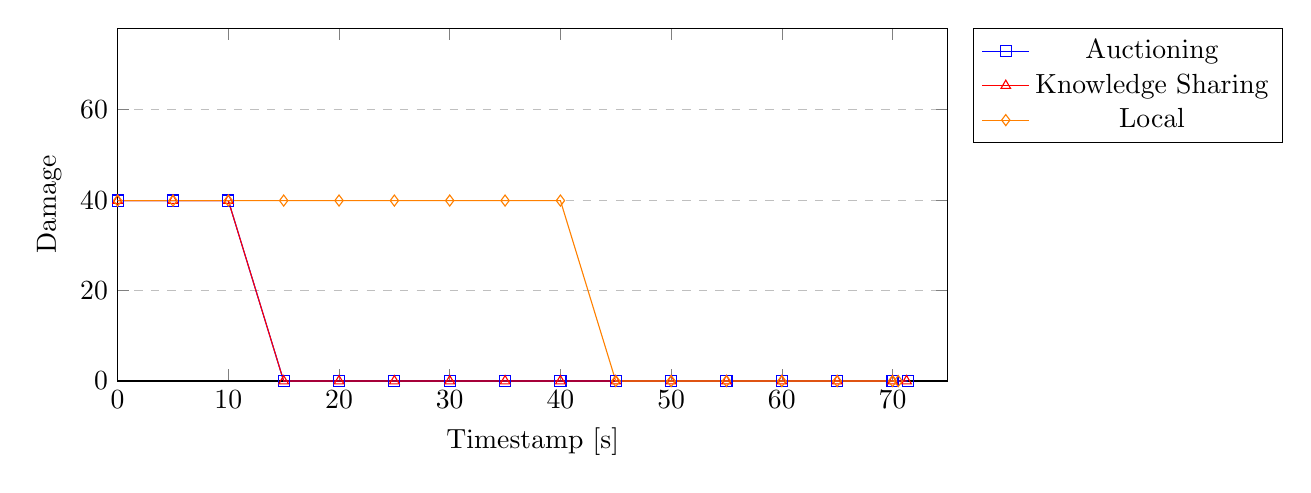
\begin{tikzpicture}
\begin{axis}[
    xlabel={Timestamp [s]},
    ylabel={Damage},
    xmin=0, xmax=75000,
    ymin=0, ymax=78,
    legend pos=outer north east,
    ymajorgrids=true,
    grid style=dashed,
    width=\textwidth,
    height=0.5\textwidth,
    scaled x ticks=base 10:-3,
    xtick scale label code/.code={}
]

	\addplot[color=blue,mark=square] coordinates {
        (0,39.90)(5000,39.90)(10000,39.90)(15000,0.00)(20000,0.00)(25000,0.00)(30000,0.00)(35000,0.00)(40000,0.00)(45000,0.00)(50000,0.00)(55000,0.00)(60000,0.00)(65000,0.00)(70000,0.00)(71384,0.00)
    };
    \addlegendentry{Auctioning}
	\addplot[color=red,mark=triangle] coordinates {
        (0,39.90)(5000,39.90)(10000,39.90)(15000,0.00)(20000,0.00)(25000,0.00)(30000,0.00)(35000,0.00)(40000,0.00)(45000,0.00)(50000,0.00)(55000,0.00)(60000,0.00)(65000,0.00)(70000,0.00)(71269,0.00)
    };
    \addlegendentry{Knowledge Sharing}
	\addplot[color=orange,mark=diamond] coordinates {
        (0,39.90)(5000,39.90)(10000,39.90)(15000,39.90)(20000,39.90)(25000,39.90)(30000,39.90)(35000,39.90)(40000,39.90)(45000,0.00)(50000,0.00)(55000,0.00)(60000,0.00)(65000,0.00)(70000,0.00)(70516,0.00)
    };
    \addlegendentry{Local}




\end{axis}
\end{tikzpicture}
    \caption{Graph showing the output of all feature sets in the non-changing scenario, with a large infrastructure.}
    \label{fig:large-infra-large}
\end{figure}

% \add{Mention the spread in consecutive runs}
% \add{Mention the performance of knowledge-sharing in smaller networks}

\subsection{Consistency}
\label{ssec:consecutive-runs}
During some of the experiments we see a small fluctuation in the behavior of agents. One good example of this is figure \ref{fig:adapting-time-no-change} compared to \ref{fig:adapting-time-risk-introduction}. We believe this is because of the scheduling of threads by the OS. This could lead into different auctions being initiated and joined over multiple runs. 

To test this assumption, we ran the no-change scenario with the auctioning feature-set $5$ times. The results of this can be seen in figure \ref{fig:multi-run-no-change}. We see that the overall damage is very similar in all runs. However, small differences can be observed across the runs.

\begin{figure}[H]
    \centering
        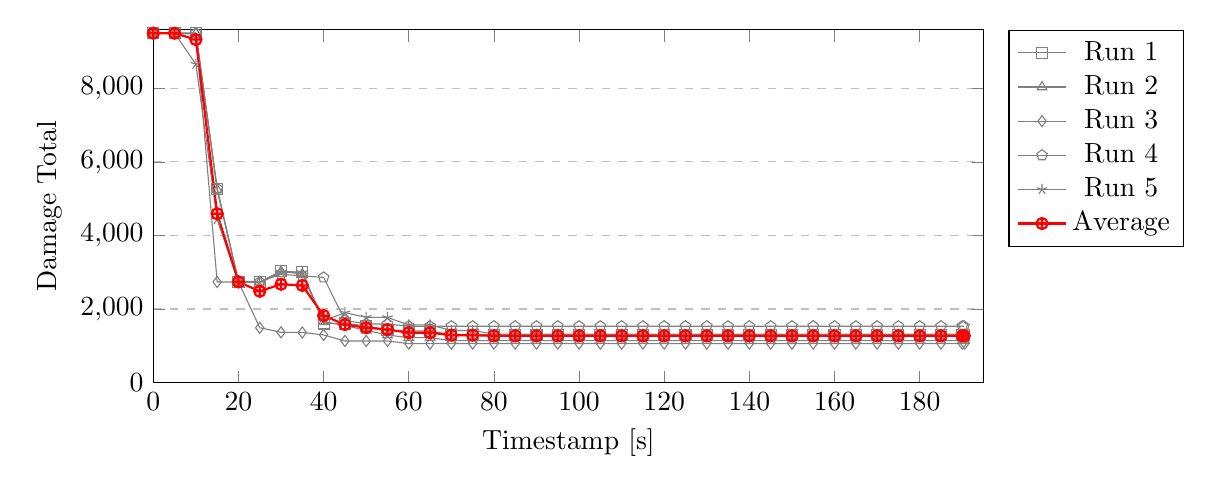
\begin{tikzpicture}
\begin{axis}[
    xlabel={Timestamp [s]},
    ylabel={Damage Total},
    xmin=0, xmax=195000,
    ymin=0, ymax=9595,
    legend pos=outer north east,
    ymajorgrids=true,
    grid style=dashed,
    width=\textwidth,
    height=0.5\textwidth,
    scaled x ticks=base 10:-3,
    xtick scale label code/.code={}
]

	\addplot[color=gray,mark=square] coordinates {
        (0,9500.86)(5000,9500.86)(10000,9500.86)(15000,5273.46)(20000,2735.67)(25000,2733.78)(30000,3030.23)(35000,2999.27)(40000,1606.26)(45000,1606.26)(50000,1545.84)(55000,1424.29)(60000,1401.35)(65000,1401.35)(70000,1299.55)(75000,1299.55)(80000,1299.55)(85000,1299.55)(90000,1299.55)(95000,1299.55)(100000,1299.55)(105000,1299.55)(110000,1299.55)(115000,1299.55)(120000,1299.55)(125000,1299.55)(130000,1299.55)(135000,1299.55)(140000,1299.55)(145000,1299.55)(150000,1299.55)(155000,1299.55)(160000,1299.55)(165000,1299.55)(170000,1299.55)(175000,1299.55)(180000,1299.55)(185000,1299.55)(190000,1299.55)(190469,1299.55)
    };
    \addlegendentry{Run 1}
	\addplot[color=gray,mark=triangle] coordinates {
        (0,9500.86)(5000,9500.86)(10000,9500.86)(15000,5244.51)(20000,2735.67)(25000,2733.78)(30000,3027.26)(35000,2951.72)(40000,1657.47)(45000,1550.25)(50000,1420.21)(55000,1293.76)(60000,1220.39)(65000,1220.39)(70000,1142.59)(75000,1142.59)(80000,1142.59)(85000,1142.59)(90000,1142.59)(95000,1142.59)(100000,1142.59)(105000,1142.59)(110000,1142.59)(115000,1142.59)(120000,1142.59)(125000,1142.59)(130000,1142.59)(135000,1142.59)(140000,1142.59)(145000,1142.59)(150000,1142.59)(155000,1142.59)(160000,1142.59)(165000,1142.59)(170000,1142.59)(175000,1142.59)(180000,1142.59)(185000,1142.59)(190000,1142.59)(190603,1142.59)
    };
    \addlegendentry{Run 2}
	\addplot[color=gray,mark=diamond] coordinates {
        (0,9500.86)(5000,9500.86)(10000,9475.27)(15000,2735.67)(20000,2735.67)(25000,1491.74)(30000,1368.06)(35000,1362.13)(40000,1296.28)(45000,1131.00)(50000,1131.00)(55000,1131.00)(60000,1059.17)(65000,1059.17)(70000,1059.17)(75000,1059.17)(80000,1059.17)(85000,1059.17)(90000,1059.17)(95000,1059.17)(100000,1059.17)(105000,1059.17)(110000,1059.17)(115000,1059.17)(120000,1059.17)(125000,1059.17)(130000,1059.17)(135000,1059.17)(140000,1059.17)(145000,1059.17)(150000,1059.17)(155000,1059.17)(160000,1059.17)(165000,1059.17)(170000,1059.17)(175000,1059.17)(180000,1059.17)(185000,1059.17)(190000,1059.17)(190583,1059.17)
    };
    \addlegendentry{Run 3}
	\addplot[color=gray,mark=pentagon] coordinates {
        (0,9500.86)(5000,9500.86)(10000,9500.86)(15000,5273.46)(20000,2757.80)(25000,2735.67)(30000,2946.76)(35000,2901.60)(40000,2859.47)(45000,1695.56)(50000,1592.95)(55000,1592.95)(60000,1531.57)(65000,1531.57)(70000,1531.57)(75000,1531.57)(80000,1531.57)(85000,1531.57)(90000,1531.57)(95000,1531.57)(100000,1531.57)(105000,1531.57)(110000,1531.57)(115000,1531.57)(120000,1531.57)(125000,1531.57)(130000,1531.57)(135000,1531.57)(140000,1531.57)(145000,1531.57)(150000,1531.57)(155000,1531.57)(160000,1531.57)(165000,1531.57)(170000,1531.57)(175000,1531.57)(180000,1531.57)(185000,1531.57)(190000,1531.57)(190405,1531.57)
    };
    \addlegendentry{Run 4}
	\addplot[color=gray,mark=star] coordinates {
        (0,9500.86)(5000,9500.86)(10000,8658.83)(15000,4434.90)(20000,2726.22)(25000,2726.22)(30000,3000.82)(35000,2997.05)(40000,1685.04)(45000,1899.99)(50000,1777.19)(55000,1769.17)(60000,1569.23)(65000,1569.23)(70000,1417.12)(75000,1417.12)(80000,1318.25)(85000,1318.25)(90000,1318.25)(95000,1318.25)(100000,1318.25)(105000,1318.25)(110000,1318.25)(115000,1318.25)(120000,1318.25)(125000,1318.25)(130000,1318.25)(135000,1318.25)(140000,1318.25)(145000,1318.25)(150000,1318.25)(155000,1318.25)(160000,1318.25)(165000,1318.25)(170000,1318.25)(175000,1318.25)(180000,1318.25)(185000,1318.25)(190000,1318.25)(190567,1318.25)
    };
    \addlegendentry{Run 5}
	\addplot[color=red,mark=oplus,thick] coordinates {
        (0,9500)(5000,9500)(10000,9326.6)(15000,4591.8)(20000,2737.6)(25000,2483.6)(30000,2674.2)(35000,2642)(40000,1820.6)(45000,1576.2)(50000,1493)(55000,1441.8)(60000,1356)(65000,1356)(70000,1289.6)(75000,1289.6)(80000,1269.8)(85000,1269.8)(90000,1269.8)(95000,1269.8)(100000,1269.8)(105000,1269.8)(110000,1269.8)(115000,1269.8)(120000,1269.8)(125000,1269.8)(130000,1269.8)(135000,1269.8)(140000,1269.8)(145000,1269.8)(150000,1269.8)(155000,1269.8)(160000,1269.8)(165000,1269.8)(170000,1269.8)(175000,1269.8)(180000,1269.8)(185000,1269.8)(190000,1269.8)(190469,1269.8)
    };
    \addlegendentry{Average}
\end{axis}
\end{tikzpicture}

    \caption{Graph showing the Auctioning Feature's performance over multiple runs in the no-change scenario.}
    \label{fig:multi-run-no-change}
\end{figure}

The metrics that are collected are not enough to fully pin-point this behavior to scheduling. but, the results seem to indicate that the variety in the performance of the agents is small, and no further investigation has been performed. However, The result from figure \ref{fig:multi-run-no-change} are positive, as it means that the agents are able to perform consistently over multiple runs.

